\documentclass[a4paper,11pt]{article}

\usepackage[utf8x]{inputenc}
\usepackage[T1]{fontenc}
\usepackage[spanish]{babel}
\usepackage{ucs}
\usepackage{palatino}
\usepackage{pdfpages}
%\usepackage[top=3cm,bottom=3cm,left=3cm,right=3cm]{geometry}
\usepackage{hyperref}
\bibliographystyle{plain-es}

\pagestyle{plain}

\usepackage{subfig}
\usepackage{graphicx}
\DeclareGraphicsExtensions{.pdf,.eps,.jpg,.png,.gif}

%\renewcommand{\emph}[1]{\textbf{#1}}
%\renewcommand{\familydefault}{\sfdefault}

\hypersetup{
    colorlinks = true,
    urlcolor = blue,
    linkcolor = black,
    citecolor = black,
    filecolor = black
}

%%%%%%%%%%%%%%%%%%%%%%%%%%%%%%%%%%%%%%%%%%%%%%%%%%%%%%%%%%%%

\title{Problema de balanceo de carga}
\author{Cristian \textsc{Pereyra} \and Laurent \textsc{Georget}}

\begin{document}
\maketitle
\tableofcontents

\clearpage

\section*{Introducción}

El uso de la simulación de eventos discretos permite resolver problemas que tienen una complejidad que impide alcanzar
a una solución con la análisis o la teoría de las probabilidades. Los casos típicos son problemas de ingeniería de la
producción donde las interacciones entre entidades (que pueden ser humanos, productos, máquinas, computadoras, etc.) y
la cantidad de objetos que componen el sistema completo en cualquier momento son tan complejas que resultaría imposible
manejar un modelo matemático correspondiente.

En nuestro caso, el sistema real que vamos a estudiar es un sistema de balanceo de carga en un ámbito de procesamiento
de pedidos web. Los dispositivos de balanceo de carga son \textit{routers} que reciben pedidos y los distribuyen a
servidores capaces de atenderlos. En el caso que nos interesa estudiar, consideramos servidores alojando aplicaciones
web a las que usuarios quieren acceder. Cada servidor puede atender uno solo pedido a la vez. Entonces, para permitir a
la aplicación de ser concurrente, y escalable, se usan varios servidores corriendo la misma aplicación. Del punto de
vista del usuario externo, eso no cambia nada porque accede a la aplicación conociendo la dirección de la página web.
Pero, internamente, el \textit{router} manda su pedido a determinado servidor. Así, la cantidad de servidores corriendo
la aplicación es directamente vinculado a la ``concurrencia'' de la aplicación, es decir la cantidad de clientes que
pueden ser atendidos a la vez.

Sin embargo, esa concurrencia no es necesariamente \emph{proporcional} a la cantidad de servidores. Como lo muestra la
formula de Little, la cantidad de entidades en un sistema no es igual a la cantidad de entidades en las colas más el
número de puestos de atención, sino a la cantidad de entidades en las colas más \emph{la tasa de tránsito}, es decir el
cociente entre el tiempo promedio entre dos arribos y el tiempo promedio de atención de una entidad. Además, en nuestro
caso, la mejora de la concurrencia según el aumento del número de servidores depende también de la política de
\textit{routing} elegida.

\section{Propósito y base del trabajo}

Nuestro proyecto se basa en un artículo de RapGenius, cliente del proveedor Heroku. En este artículo, RapGenius critica
el reciente cambio en la política de load-balancing de su proveedor, mostrando, con resultados de simulaciones corridas
en R, que ese cambio resulta en resultados pésimos. Según RapGenius, una empresa necesitaría
cincuenta veces más servidores corriendo la misma aplicación para alcanzar la misma disponibilidad con el nuevo modelo
de routing, muy sencillo, que la que permitía el antiguo modelo, que usaba un algoritmo más complicado.

\begin{figure}[h]
    \centering
    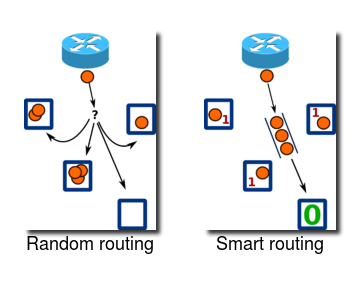
\includegraphics[height=200px]{random-smart.png}
    \caption{Los dos modelos presentados por RapGenius en su artículo}
    \label{fig:random+smart}
\end{figure}

El primer algoritmo, llamado ``Smart routing'', hace que cuando el \textit{router} recibe un pedido, lo manda a un servidor
desocupado. Si no hay, lo guarda en una cola. Cada vez que un servidor se desocupa, el pedido que llegó primero en la
cola va a este servidor. Entonces, en este modelo, no hay cola a nivel de servidores.

El segundo algoritmo se llama ``Random routing''. Es mucho más sencillo. El \textit{router} manda cada pedido que llega
a cualquier servidor. La única condición es que el servidor debe tener lugar en su cola. Si está lleno, el
\textit{router} intenta con otro servidor, hasta que encuentra un servidor o que alcanza un número máximo de intentos.
Si no logra encontrar un servidor con lugar en su cola, guarda el pedido en su propia cola.

En nuestro proyecto, el objetivo es comprobar los resultados de RapGenius y además verificar cuál podría ser el mejor
algoritmo. Por eso, estudiamos además del ``Smart routing'' y del ``Random routing'' otros dos algoritmos: el
``Round-robin routing'' y el ``Shortest queue routing'' (ver imagen \ref{fig:round_robin+shortest_queue}).

\begin{figure}[h]
    \centering
    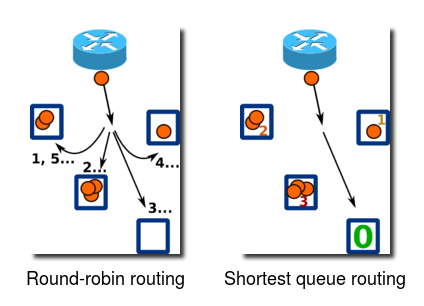
\includegraphics[height=200px]{round-robin--shortest-queue.png}
    \caption{Los otros dos modelos estudiados}
    \label{fig:round_robin+shortest_queue}
\end{figure}


El algoritmo de round-robin funciona de manera muy simple. El \textit{router} construye una lista circular\footnote{Una 
lista ``sin fin'' donde el elemento siguiente del último es el primero} de servidores y sabe a cual mandó el último pedido. 
Cuando recibe otro, lo manda al servidor siguiente en la lista, si ese tiene lugar en su cola. Si no, intenta con el
siguiente. Si ningún servidor tiene lugar, guarda el pedido en su propia cola.

Para finalizar, cuando usa el algoritmo de ``Shortest queue'', el \textit{router} manda cada pedido que llega al
servidor que tiene menos cola (o no cola) en este momento. Si hay más de un servidor con cola mínima, elige uno al
azar. Es el algoritmo más complicado de implementar, ya que requiere que el \textit{router} conozca el estado completo
de los servidores a cada momento.



\section{Modelo conceptual}

\subsection{Simplificaciones}

Nuestro modelo es una maqueta que simula el funcionamiento lógico de un verdadero balanceador de carga. Sin embargo, los
balanceadores de carga, por el papel que tienen en el funcionamiento de la red, tienen una complejidad mucha mas
importante que la de nuestro modelo. En nuestro simulador, todo el funcionamiento de la red informática es una
abstracción. El \textit{router} solamente se encarga de decidir a que servidor mandar pedidos que le llegan. No
contemplamos tampoco las fallas y los errores lógicas y materiales que pueden ocurrir en un verdadero sistema.

\subsection{Diagrama de bloques}

Nuestro sistema funciona de la manera presentada en la figura \ref{fig:diagrama-bloques}. Cuando la simulación empieza,
no hay pedidos pendientes en el sistema, y el primer pedido está llegando. Cada etapa de la simulación corresponde a un
evento, o sea un arribo de un pedido al \textit{router}, o una salida de un pedido de un servidor. En el diagrama, se
nota que cada pedido pasa por la cola del \textit{router} antes de llegar a un servidor. Sin embargo, en nuestro modelo,
hacemos la simplificación que todo el tiempo que el pedido pasa en el sistema se divide entre la espera en colas y el
procesamiento en un servidor. Los tiempos de tránsito o de \textit{routing} están considerados como despreciables.
Entonces, si es posible mandar directamente el pedido a un servidor cuando entra en la cola del \textit{router}, el
tiempo de principio de procesamiento en el servidor es igual al tiempo de llegada al \textit{router}, o sea el paso por
la cola principal no afecta el pedido en este caso.

\begin{figure}[h]
    \centering
    \includegraphics[width=\textwidth]{diagrama_bloques.png}
    \caption{Diagrama de bloques}
    \label{fig:diagrama-bloques}
\end{figure}

En la figura \ref{fig:diagrama-bloques}, el bloque más importante para nuestro estudio es el bloque en verde. La
elección del servidor puede hacerse con cualquier de los cuatro algoritmos de \textit{routing}.


\subsection{Plan de cuadros}

\subsubsection{Valores relevantes del modelo}

\paragraph{Variable de control}
En nuestro estudio, tenemos una sola variables de control: el algoritmo utilizado para elegir un servidor al que mandar
un pedido. No es una variable cuantitativa así que no se espera encontrar el mejor algoritmo en absoluto sino observar
las ventajas y desventajas de cada algoritmo de forma objetiva.

\paragraph{Funciones objetivos}
Contemplamos varios resultados:
\begin{itemize}
    \item el tiempo promedio que un pedido pasa en el sistema, entre el momento en que llega al \textit{router} hasta el
	momento en que sale del servidor que lo atendió
    \item el tiempo ocioso promedio de un servidor
    \item el número de pedidos rechazados
\end{itemize}
De la segunda función, se estudia también el desvío entre servidores. Una calidad que se busca en un balanceador de
carga es la equidad: es decir, todos los servidores deberían tener una carga parecida.


\paragraph{Parámetros}
Algunos valores pueden afectar la simulación. Eses parámetros son los siguientes:
\begin{itemize}
    \item el número de servidores
    \item el tamaño máximo de la cola de \textit{router}
    \item el tamaño máximo de la cola de cada servidor, en el caso de \textit{Smart routing}, no hay colas en los servidores
    \item la cantidad de corridas
\end{itemize}


\subsubsection{Resultados esperados}

\begin{table}
    \centering
    \begin{tabulary}{\textwidth}{|c||C||C|C|C|}
    \hline
    Algoritmo & Número de servidores & Duración promedia de un pedido & Tiempo ocioso promedio & Desvío entre servidores del tiempo ocioso \\
    \hline
	\multirow{4}{1.8cm}{Random routing} & 30 &  &  &  \\
                                        & 40 &  &  &  \\
                                        & 50 &  &  &  \\
                                        & 60 &  &  &  \\
	\hline
    \multirow{4}{1.8cm}{Round-robin routing} & 30 &  &  &  \\
                                             & 40 &  &  &  \\
                                             & 50 &  &  &  \\
                                             & 60 &  &  &  \\
	\hline
    \multirow{4}{1.8cm}{Shortest queue routing} & 30 &  &  &  \\
                                                & 40 &  &  &  \\
                                                & 50 &  &  &  \\
                                                & 60 &  &  &  \\
	\hline
    \multirow{4}{1.8cm}{Smart routing} & 30 &  &  &  \\
                                       & 40 &  &  &  \\
                                       & 50 &  &  &  \\
                                       & 60 &  &  &  \\
	\hline
    \end{tabulary}
    \caption{Cuadro comprativo de los resultados esperados}
    \label{tab:plan-cuadros}
\end{table}



Los resultados que esperamos están presentados en el cuadro \ref{tab:comparativo-esperados}. Este cuadro se lee de la 
siguiente manera: para ciertos criterios, que consideramos relevantes, hicimos una clasificación de los algoritmos. Para
cada criterio, el algoritmo clasificado como ``1'' es el mejor, y el ``4'' el peor. 

\begin{table}
    \centering
    \begin{tabulary}{\textwidth}{|c||C|C|C|}
    \hline
    Algoritmo & Complejidad  de implementación & Equidad en la ocupación & Duración promedia de un pedido \\
    \hline
	Random routing & 2 & 4 & 4\\
	\hline
	Round-robin routing & 1 & 3 & 3\\
	\hline
	Shortest queue routing & 4 & 1 & 2\\
	\hline
	Smart routing & 3 & 2 & 1\\
	\hline
    \end{tabulary}
    \caption{Cuadro comprativo de los resultados esperados}
    \label{tab:comparativo-esperados}
\end{table}

\subsection{Diagrama de flujo}

%falta el diagrama de flujo por acá
Tomamos la decisión de incluir en el diagrama de flujo únicamente la lógica del modelo,
olvidándonos a propósito de las ecuaciones y de los pasos que describen la colección de los
datos estadísticos. La motivación principal para eso es aliviar lo más posible el diagrama
para hacer hincapié en la lógica. Además, si bien un diagrama de flujo describe con exactitud
la lógica de un algoritmo, no sirve para diseñar el almacenamiento de los datos, y esta parte
tiene demasiada importancia a la hora de describir la colección de datos estadísticos para
ignorarla.



%\section{Modelo de datos}

A los dos tipos de eventos que contemplamos en nuestro modelo corresponden dos muestras artificiales.
La primera variable aleatoria sirve para definir los tiempos entre llegadas, la segunda para los 
tiempos de procesamiento de los pedidos en los servidores. Para definir las distribuciones de esas
variables aleatorias, nos basamos en el artículo de RapGenius. Ellos estudiaron las distribuciones
de llegadas y de salidas en su propio caso y utilizar los mismos datos nos permite comparar nuestros
resultados con los suyos.

\paragraph{Distribución de tiempo entre llegadas}
Los pedidos llegan al \textit{router} según un proceso de Poisson. Según RapGenius, hay un promedio
de nueve mil pedidos por minutos. Elegimos como unidad de tiempo en todo el modelo la milisegundo;
entonces nuestra primera muestra artificial usa una distribución de Poisson de parámetro 
$\lambda = 6.667 \mathrm{ms}$.

\paragraph{Distribución de tiempo de procesamiento}
En el ámbito de aplicaciones web, la amplitud del intervalo de los tiempos de procesamiento 
es muy grande. 
Según RapGenius, el tiempo mínimo es de $10\mathrm{ms}$ y el máximo de $30000\mathrm{ms}$.
La distribución acumulada de los tiempos es la siguiente:
\begin{table}
    \centering
    \begin{tabulary}{\textwidth}{|C|C|C|C|C|C|C|C|C|}
        \hline
        1\% & 5\% & 10\% & 25\% & 50\% & 75\% & 90\% & 99\% & 99.9\% \\
        \hline
        7ms & 8ms & 13ms & 23ms & 46ms & 255ms & 923ms & 3144ms & 7962ms \\
        \hline
    \end{tabulary}
    \caption{Distribución de los tiempos de procesamiento}
    \label{tab:distro-procesamiento}
\end{table}
Esta distribución se aproxima muy bien con $Weibull(shape=0.46,\;scale=111)$ modificada
para tener en cuenta un mínimo de $10\mathrm{ms}$ y un máximo de $30000\mathrm{ms}$.

%\section{Modelo operacional}

\subsection{Simulador}

Nuestro simulador es una aplicación web basada en el \textit{framework} \emph{Ruby on Rails}.
Consta de dos partes: el núcleo que se encarga de correr la simulación y colectar los resultados
y la página web que presenta los resultados y la animación de la simulación.
El núcleo está programado en \emph{Ruby} y la animación de la página web en \emph{JavaScript}.


El simulador sigue exactamente la lógica del diagrama de flujo pero viene además con funciones
para la colección de datos estadísticos. Ruby es un lenguaje orientado a objetos y de muy alto
nivel, lo que nos permitió centrarnos en la lógica del algoritmo. El núcleo se comunica con la
parte de presentación a través de un documento en el formato ``json''. Este formato es muy
simple y permite el intercambio de datos de proceso a proceso de manera muy eficiente.


% acá, podemos describir un poco la UI

\subsection{Plan de experimentación}

Nuestro plan de experimentación sigue basicamente el plan de cuadros


%\input{resultados}
%\section*{Conclusión}

La simulación de eventos discretos sirve para encontrar soluciones, a veces
aproximadas, a problemas que no se pueden resolver analíticamente o solamente
con los herramientas de la estadística. Sin embargo, es un método muy formal,
que requiere un gran rigor, para que permita sacar conclusiones y recomendaciones
relevantes. Su otra ventaja es que, además de los resultados, la simulación suele
presentar resultados gráficos que permiten entender mejor el funcionamiento del
sistema, ver donde quedan los cuellos de botella, estudiar las interacciones
que no se pueden predecir en un modelo matemático, etc.

% me falta un poco de chamullo mágico acá a propósito de los resultados

La elección de Ruby on Rails para desarrollar el simulador resultó una 
experimentación muy útil y muy positiva. El lenguaje Ruby, por ser mucho más
lento que Java o C++, no se usa para proyectos de SED muy grandes. 
El mayor problema es la escalabilidad: Ruby no permite, por su construcción,
manejar simulaciones con miles de entidades a la vez y grandes colecciones de datos.
Sin embargo, para estudios sobre sistemas bastante pequeños y que no requieren 
una cantidad increíbles de corridas, la facilidad de programación de Ruby 
es una ventaja enorme. 




\clearpage
%\bibliography{../../../biblio}
\end{document}
